\begin{columns}
    \begin{column}{0.5\textwidth}\centering
    \begin{figure}[!htbp]
    \begin{center}
    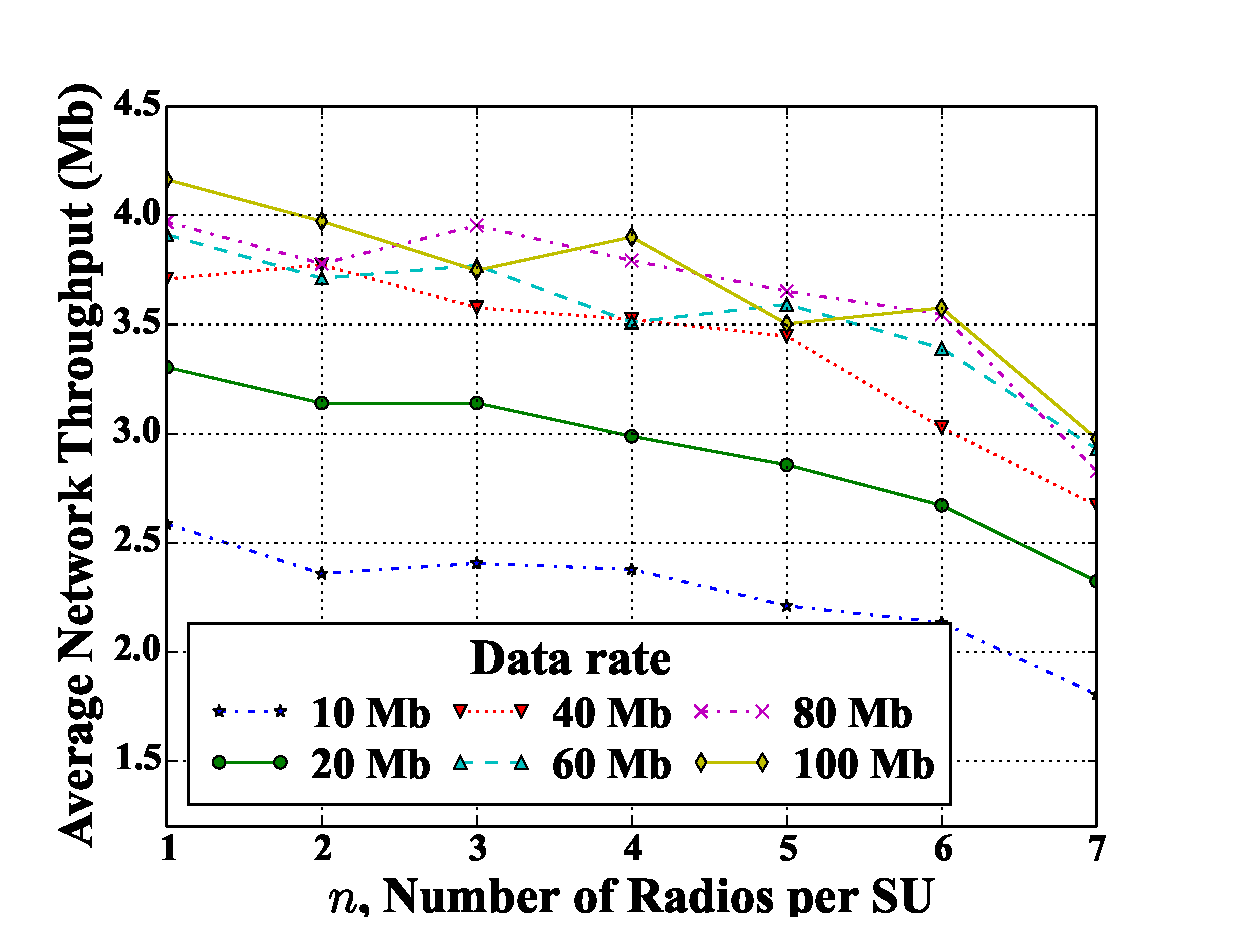
\includegraphics[scale=0.25]{figures/throughput_backup_datarate}
    \caption{Back-up Approach}
    %\caption{delay \textcolor{blue}{improves} up to a certain point, and then start to degrade}
    %\label{fig:layer}
    \end{center}
    \end{figure}
    \end{column}
    \begin{column}{0.5\textwidth}\centering
    \begin{figure}[!htbp]
    \begin{center}
    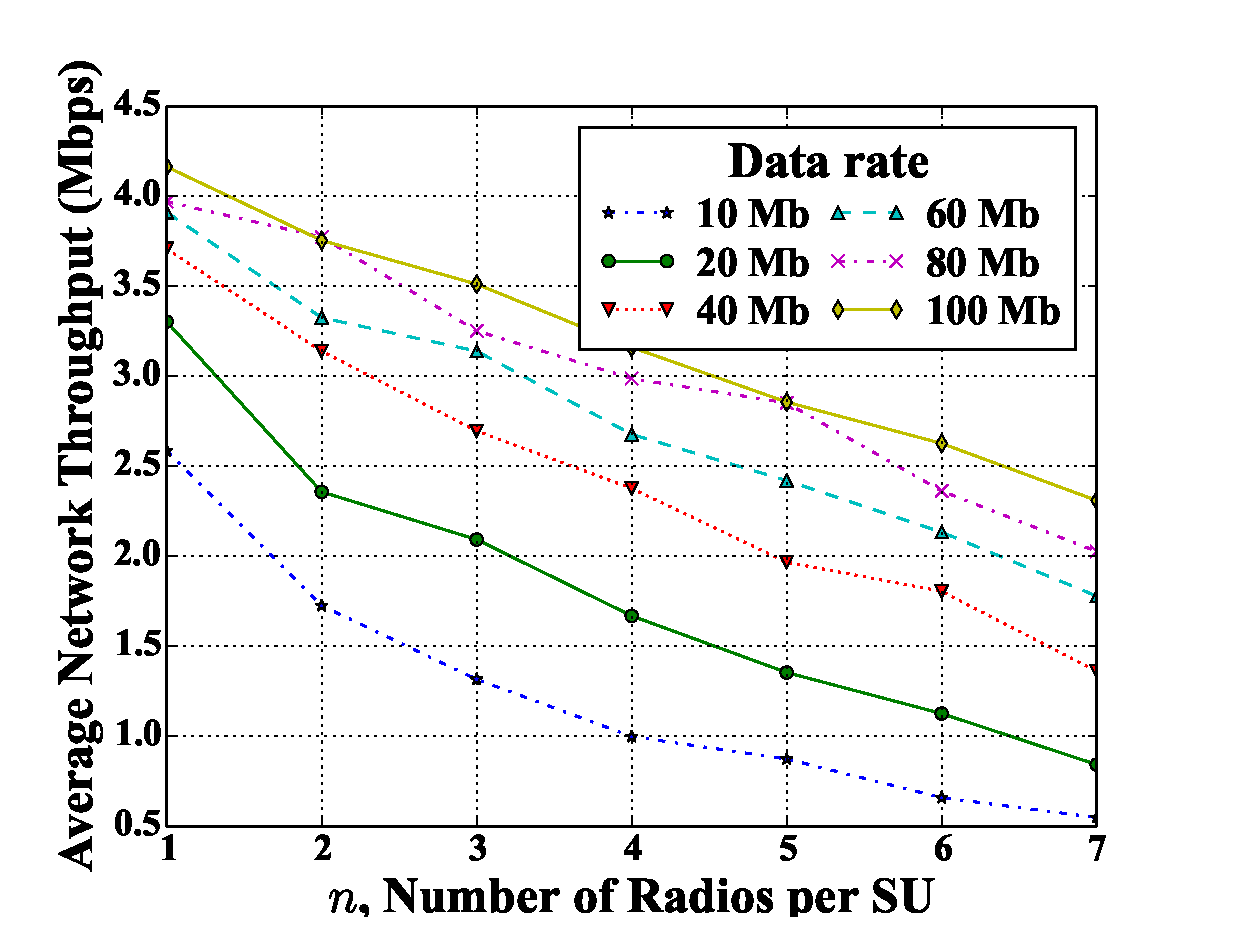
\includegraphics[scale=0.25]{figures/throughput_fragmented_datarate}
    \caption{Fragmented Approach}
    %\caption{delay \textcolor{blue}{improves} up to a certain point, and then start to degrade}
    %\label{fig:layer}
    \end{center}
    \end{figure}
    \end{column}
\end{columns}
\begin{center}
%\only<1>{\textcolor{blue}{backup} approach generally performs better}
\only<1>{Throughput always \textcolor{red}{degrades} with an increase in number of radios per SU\\
In case of Back-up approach, the degradation is lower.}
\end{center}
